% Source: TeX Live PGF manual, pgfmanual-en-tikz-trees.tex.
\documentclass[border=2pt]{standalone}
\usepackage{tikz}
\usetikzlibrary{trees}

\begin{document}
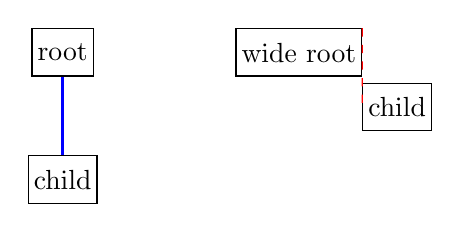
\begin{tikzpicture}[
  level distance=1cm,
  every node/.style={rectangle,draw,minimum height=6mm,inner sep=2pt},
  every child node/.style={anchor=north}
]
  \node (south) at (0,0) {root}
    [growth parent anchor=south,parent anchor=south,child anchor=north]
    child {node {child} edge from parent[blue,thick]};

  \node (northeast) at (3,0) {wide root}
    [growth parent anchor=north east,parent anchor=north east,child anchor=west]
    child {node[anchor=west] {child} edge from parent[red,dashed]};
\end{tikzpicture}
\end{document}
